\chapter{Resultados}\label{chap:resultados}

\section{Encoder}\label{sec:res-encoder}

    \begin{figure}[H]
        \centering
        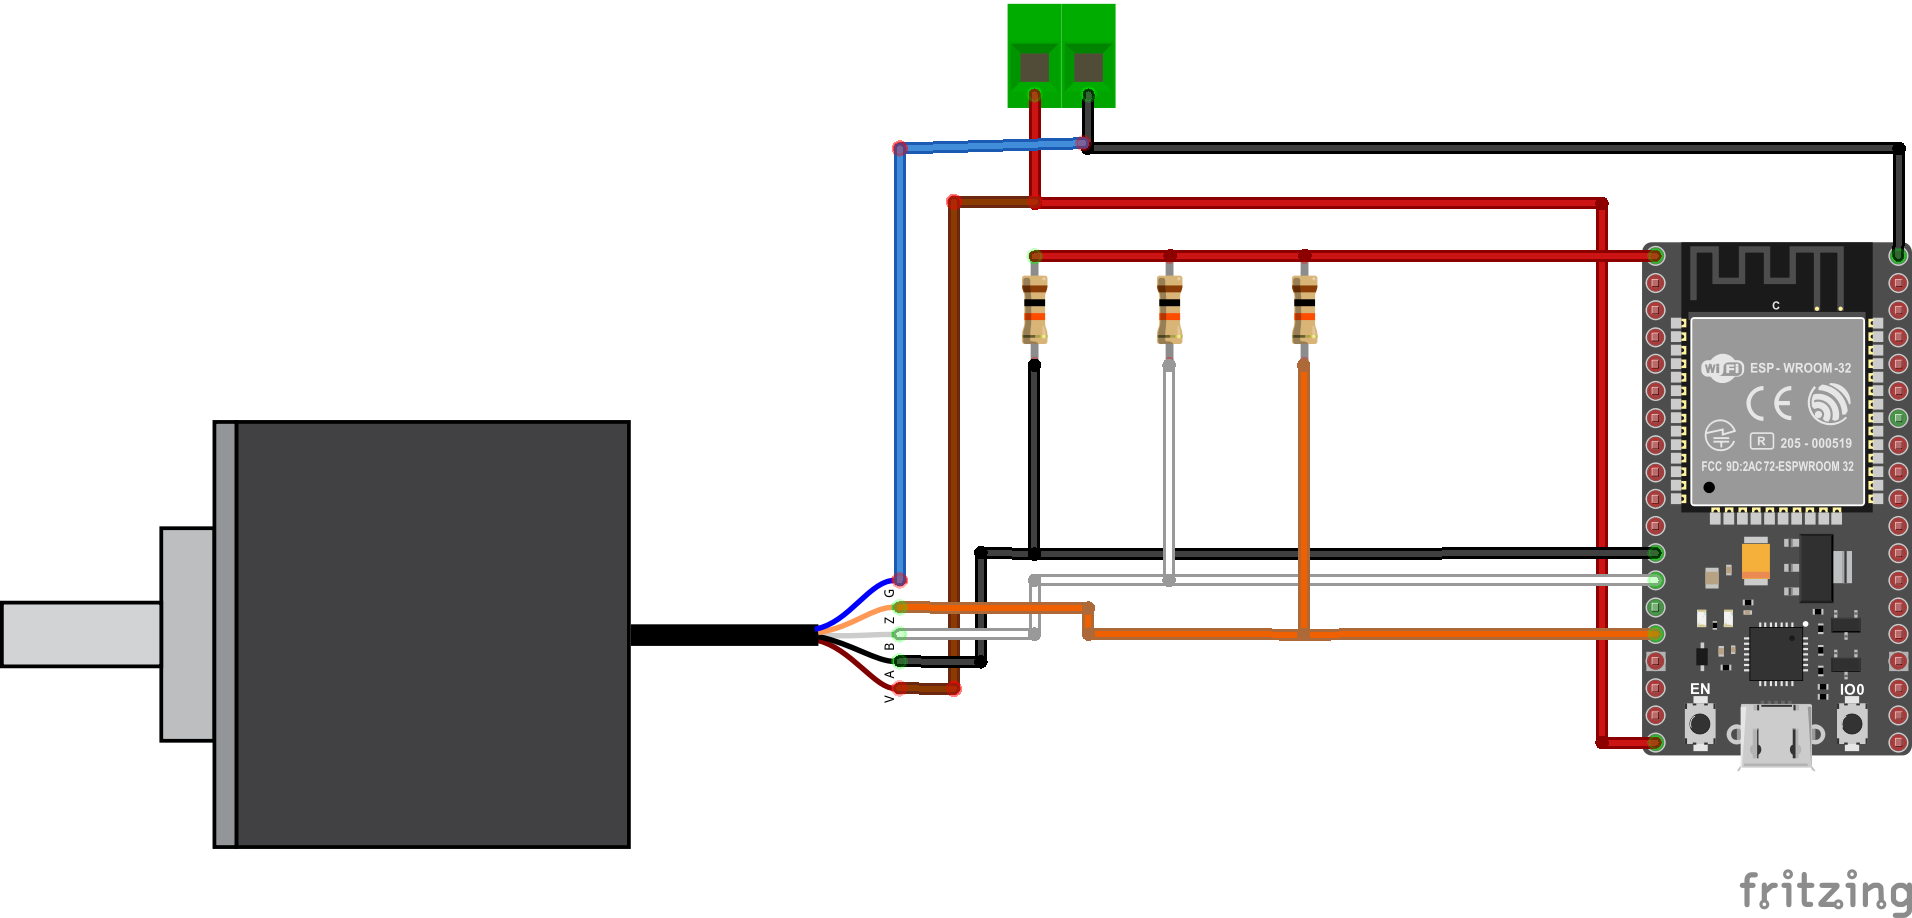
\includegraphics[width=\textwidth]{04-figuras/diagrama_conexion_encoder_bb.png}
        \caption{Diagrama de conexiones de integración encoder y esp32.}
        \label{fig:conexiones-encoder}
    \end{figure}

    \begin{itemize}
        \item \textbf{main.c implementando libreria "encoder"} \ref{cod:lib_encoder}
        \verbatiminput{07-Códigos/maine.c}
    \end{itemize}

\section{Motor}\label{sec:res-motor}

    \begin{figure}[H]
        \centering
        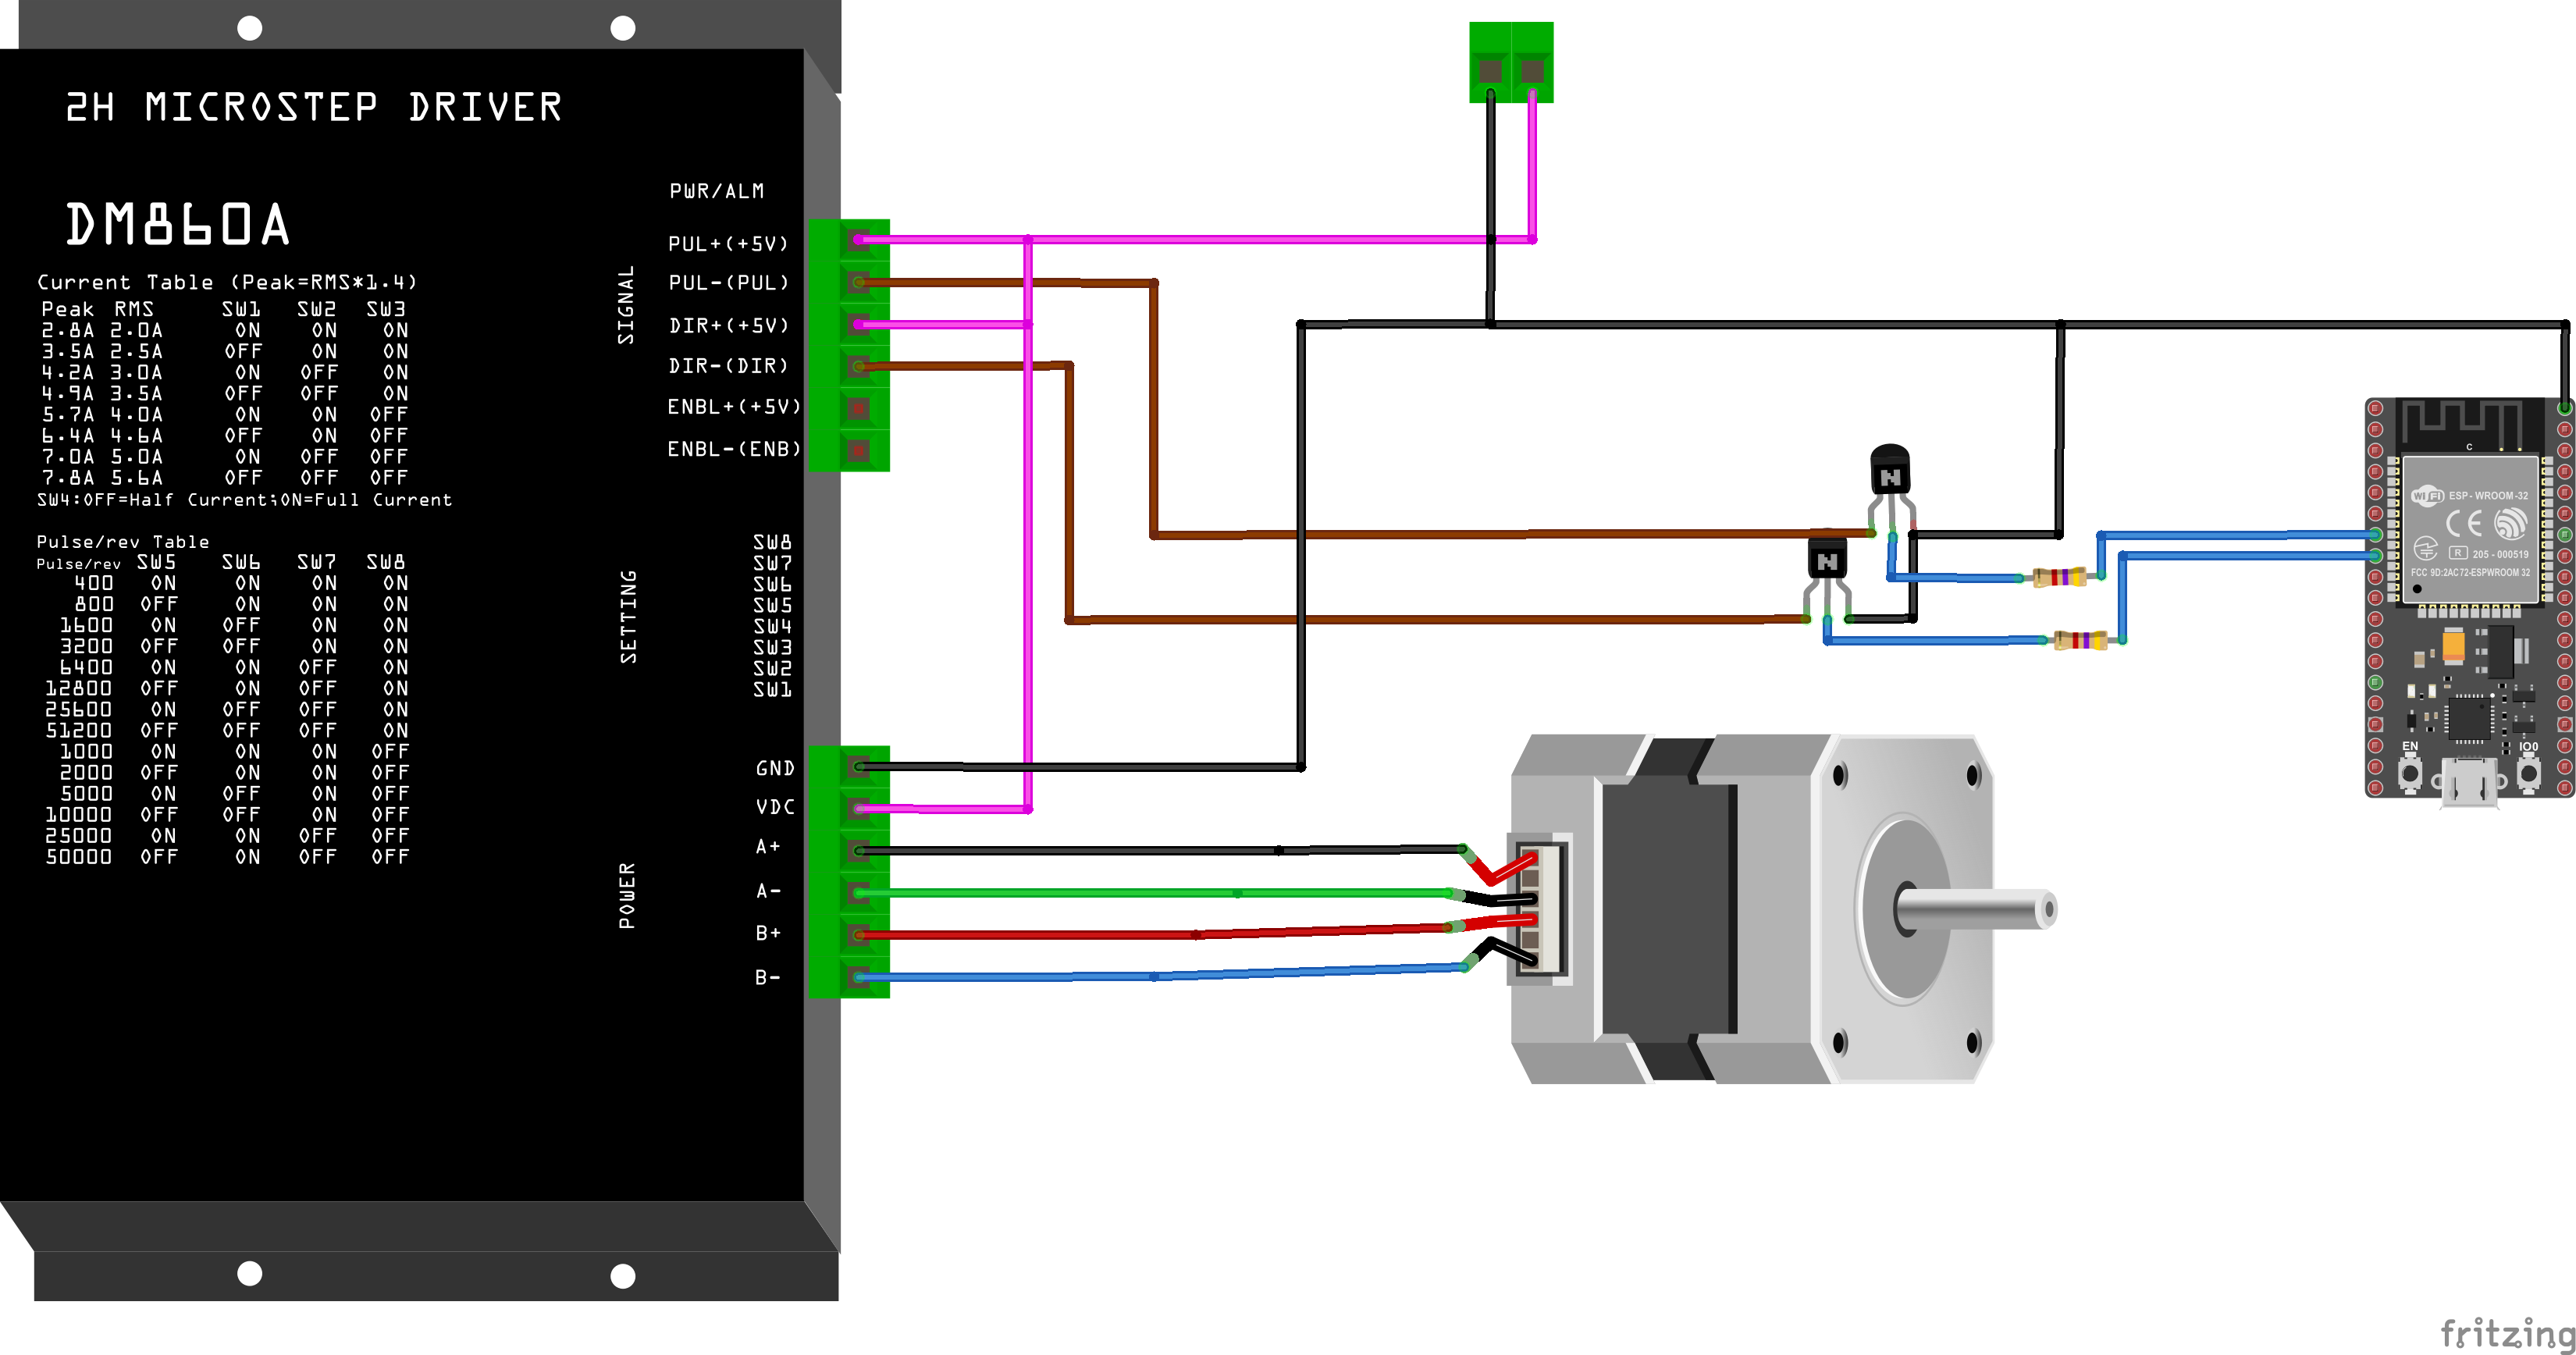
\includegraphics[width=\textwidth]{04-figuras/diagrama_conexion_motor_bb.png}
        \caption{Diagrama de conexiones driver y motor, en conjunto con el esp32.}
        \label{fig:conexiones-motor}
    \end{figure}

    \begin{itemize}
        \item \textbf{main.c implementando libreria "stepperMotor"} \ref{cod:lib_stepperMotor}
        \verbatiminput{07-Códigos/mainm.c}
    \end{itemize}

\section{Modulo de trabajo}

    \begin{figure}[H]
        \centering
        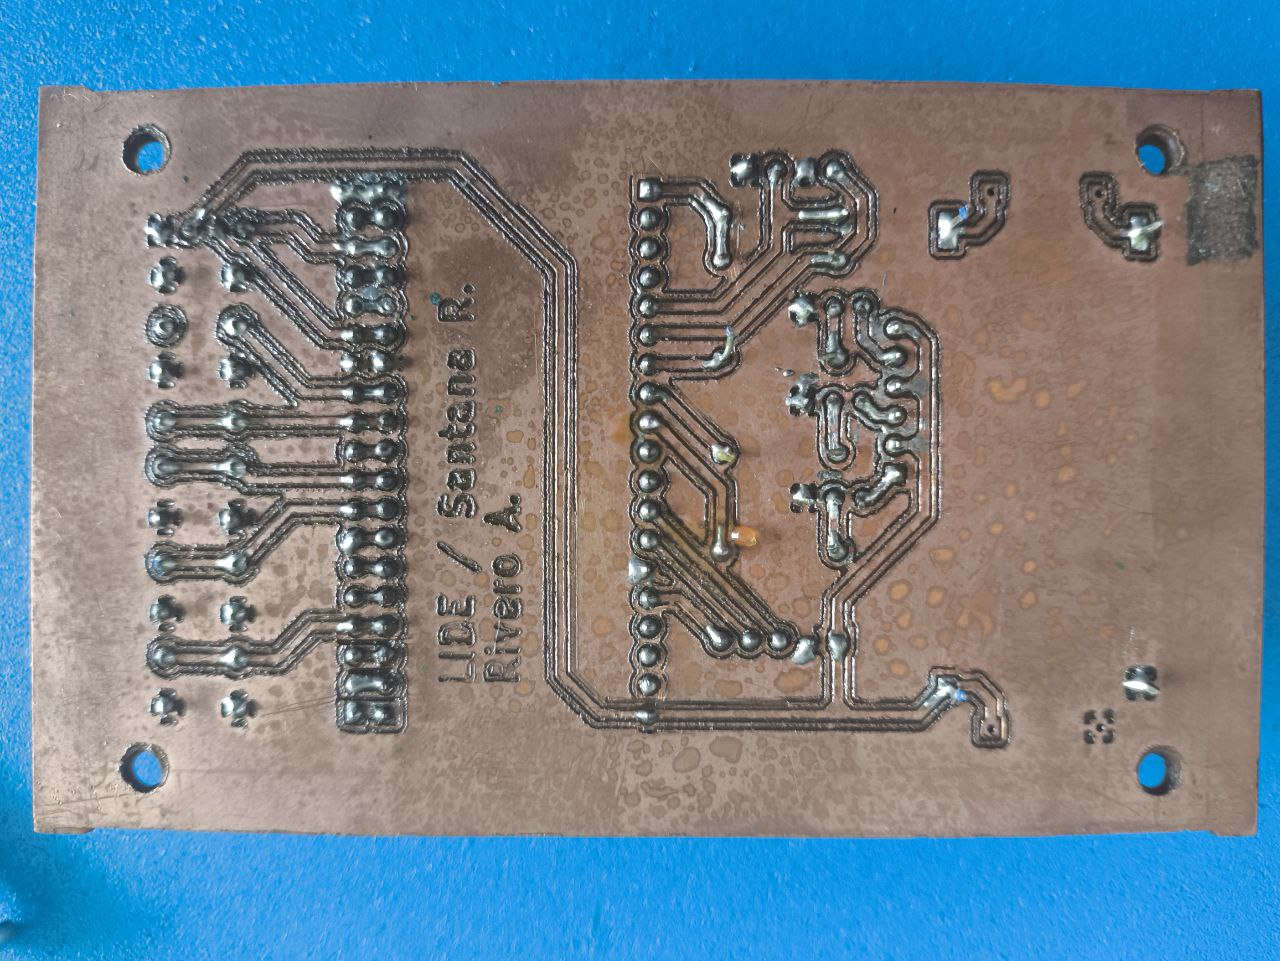
\includegraphics[height=5cm]{04-figuras/placaB.jpg}
        \caption{Vista inferior de modulo de trabajo basado en esp32.}
        \label{fig:placaB}
    \end{figure}

    \begin{figure}[H]
        \centering
        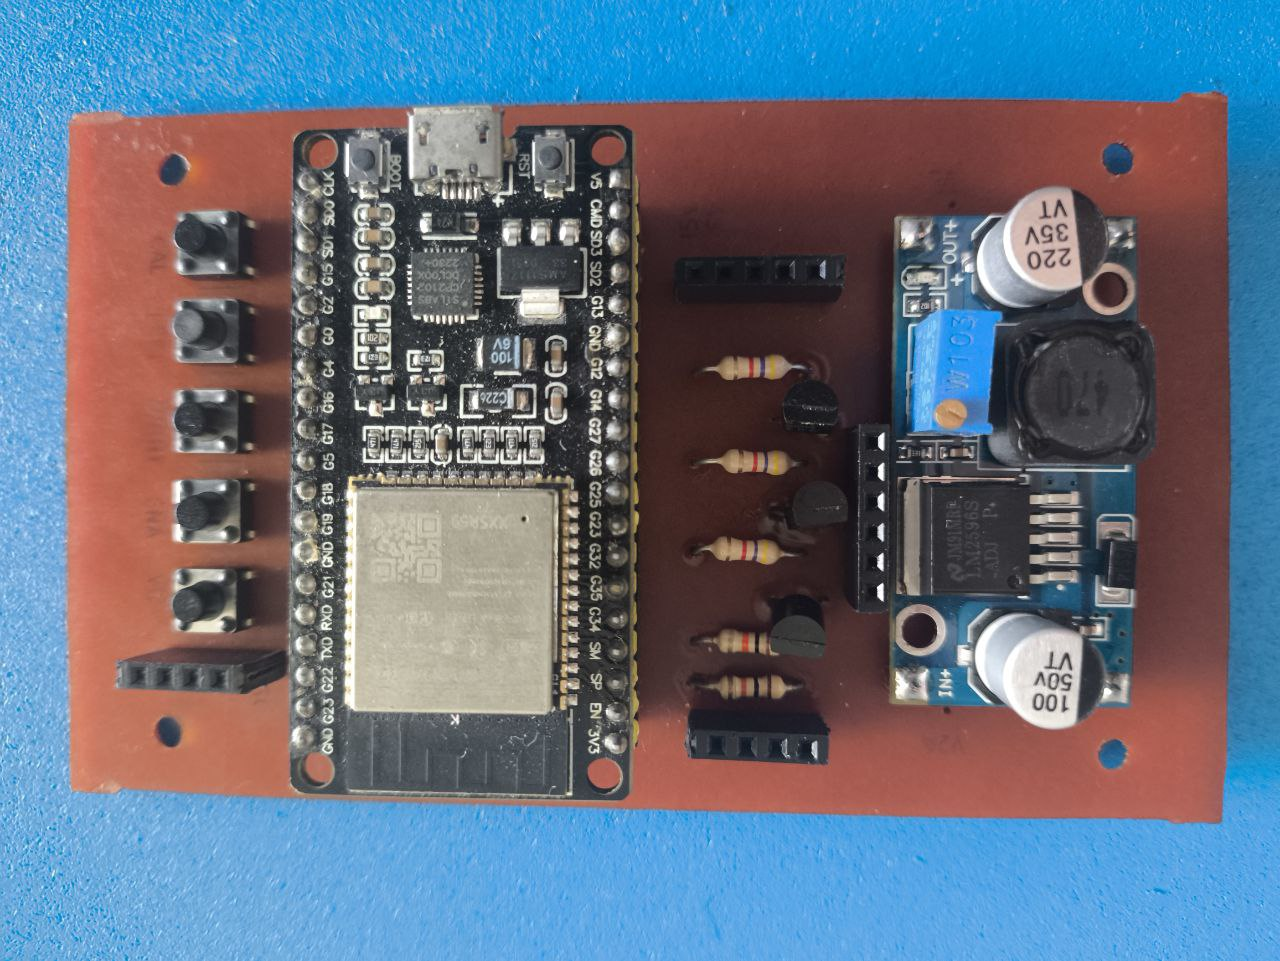
\includegraphics[height=5cm]{04-figuras/placaF.jpg}
        \caption{Vista superior de modulo de trabajo basado en esp32.}
        \label{fig:placaF}
    \end{figure}

\section{diagrama de conexiones aplicación.}

    \begin{figure}[H]
        \centering
        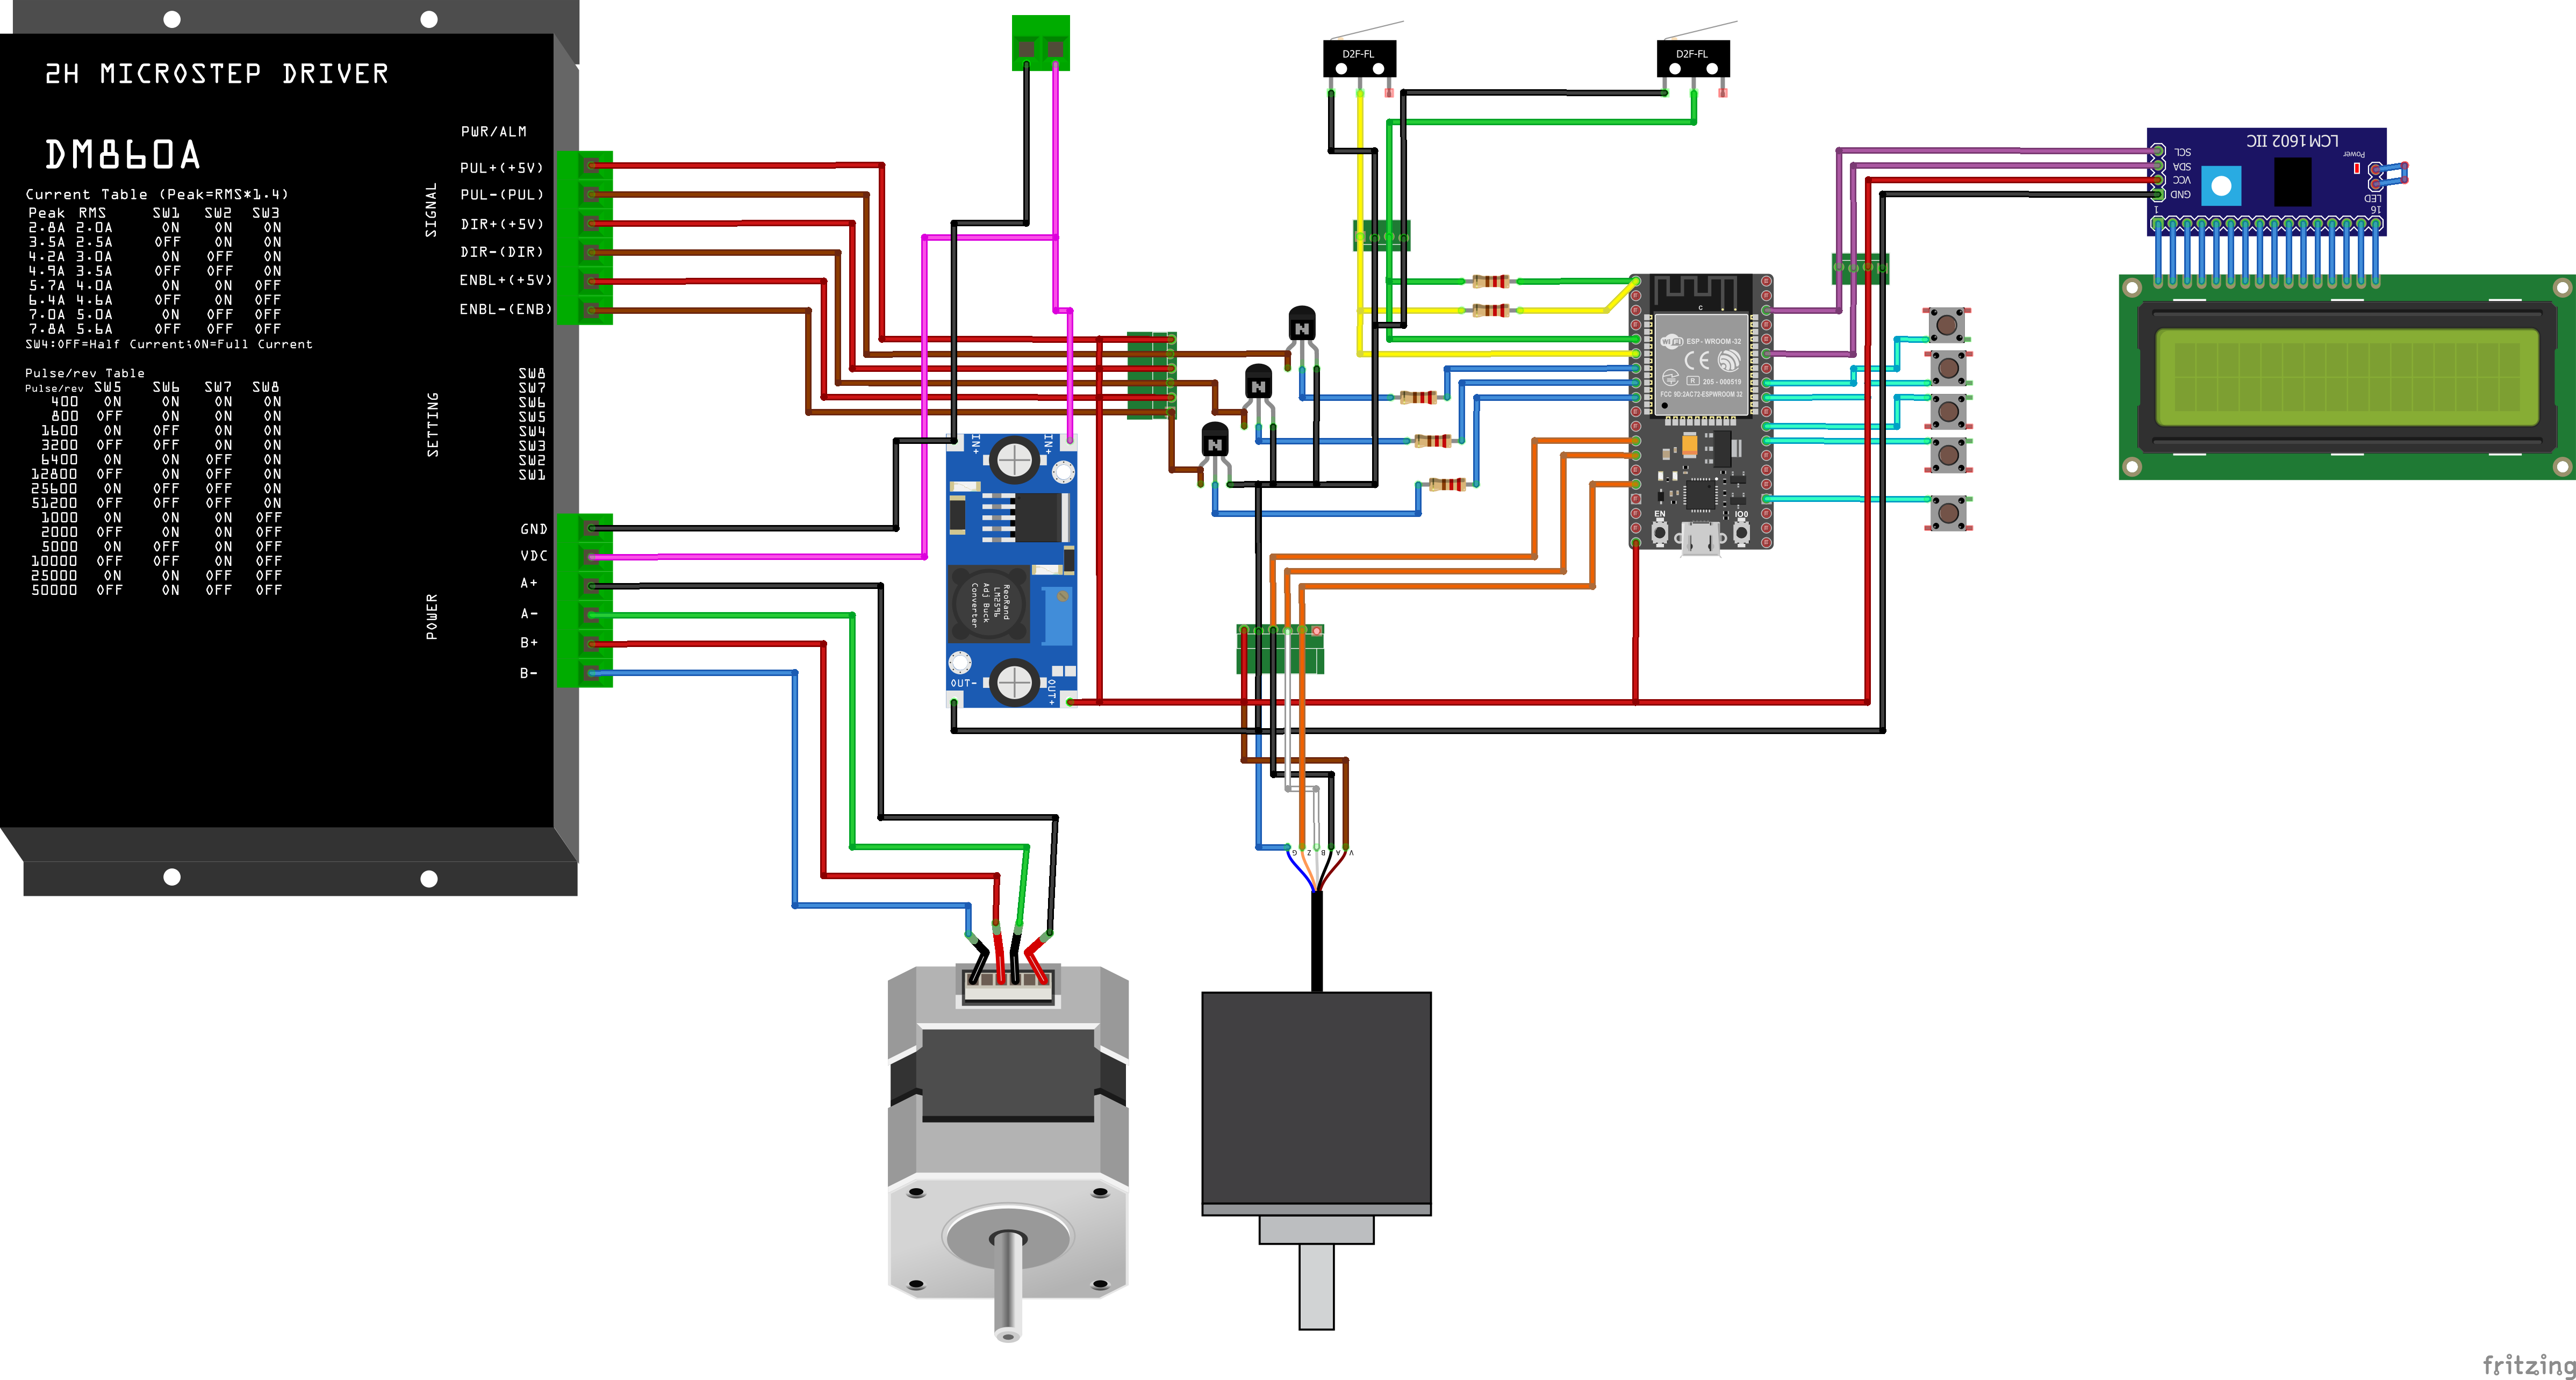
\includegraphics[width=\textwidth]{04-figuras/diagrama_conexion_control_bb.png}
        \caption{Diagrama de conexiones de sistema.}
        \label{fig:diagrama-completo}
    \end{figure}